% basic nastaveni
\documentclass[12pt]{article}
\setlength{\parindent}{0pt}
\setlength{\parskip}{1em}
\usepackage[utf8]{inputenc}
\usepackage[czech]{babel}
\usepackage[T1]{fontenc}
\usepackage{graphics}
\usepackage{caption}
\usepackage{hyperref}
\usepackage{float}

% matematicke package
\usepackage{amsmath}
\usepackage{amsfonts}
\usepackage{amssymb}
\usepackage{geometry}
\geometry{margin=2.5cm}
\usepackage{pgfplots}
\pgfplotsset{compat=1.18}
\usepackage{mathrsfs}

\title{Maturitní otázka číslo 14: Zobrazení v rovině}
\author{}
\date{}

\begin{document}
\maketitle

\subsection*{Co to je zobrazení}
Zobrazení $f$ v rovině je předpis, který každému bodu $X$ roviny přiřazuje právě jeden bod $X'$ této
roviny. Bod $X$ se nazývá vzor a bod $X'$ obraz. Zapisujeme to jako $f(X) = X'$ nebo $f : X
\mapsto X'$. Zobrazení se nazývá prosté právě tehdy, když každé dva různé body $X, Y$ zobrazí na dva
různé body $X', Y'$ roviny. To je důležité pokud bychom chtěli dělat zobrazení inverzní, pokud by
zobrazení neblo prosté, nešlo by zjistit původní vzor.

Máme-li zobrazení $f$ v rovině, samodružný bod je takový bod $X$, který se zobrazí sám na sebe, tedy
platí $f(X) = X$. Samodružná přímka $p$ je taková přímka, která se zobrazí do sebe sama, tedy platí
$f(p) = p$.

\subsection*{Shodná zobrazení}
Zobrazení se nazývá shodné zobrazení, pokud pro každé dva body $X, Y$ roviny a jejich obrazy $X', Y'$
platí $|XY| = |X'Y'|$. Obrazem každého geometrického útvaru je geometrický útvar shodný, tedy obraz
se dá tak přemístit, že se vzor s ním kryje. Specifickým typem shodného zobrazení je identické
zobrazení, které každému bodu $X$ roviny přiřazuje ten stejný bod $f(X) = X$.

Shodná zobrazení se dále dělí na přímou a nepřímou shodnost. Představme si trojúhelník, který ma
svoje vrcholy popsané proti směru hodinových ručiček. Příma shodnot nechá směr pojmenování
trojúhelníku stejný a patří mezi ní identita, posunutí, otočení a středová souměrnost. Nepřímá
shodnost vytvoří trojúhelník, který bude shodný, ale bude pojmenován po směru hodinových ručiček. Jde
si to představit jako kdyby ho někdo vzal a otočil jako palačinku. Mezi nepřímou shodnost patří
osová souměrnost.
\subsubsection*{Středová souměrnost}
Středová souměrnost $S(S)$ se středem v bodě $S$ je zobrazení, ve kterém se bod $S$ zobrazí na bod
$S' = S$ a každý bod $X$, který není $S$ se zobrazí tak, že bod $S$ je středem úsečky $XX'$. Platí
tedy, že $|XS| = |SX'|$. Bod $S$ se nazývá střed souměrnosti. Středová souměrnost se středem
souměrnosti v bodě $S$ se zapisuje jako $S(S) : X \mapsto X'$ a udává že bod $X'$ je obrazem bodu $X$.

Samodružným bodem středové souměrnosti je střed souměrnosti a samodružné přímky jsou všechny
přímky, které procházejí středem souměrnosti.

Při konstrukcích se často využívá to, že jsou nějaké útvary středově souměrné. Patří mezi ně
například čtverec, obdélník, kružnice, kosočtverec nebo kosodélník. Středem souměrnosti kružnice je
její střed. U ostatních vyjmenovaných útvarů je to průsečík jejich úhlopříček.
\subsubsection*{Posunutí}
Posunutí $T(AB)$ neboli translace určené orientovanou úsečkou $AB$ je zobrazení, ve kterém se zobrazí
bod $X$ na bod $X'$ tak, že orientované úsečky $AB$ a $XX'$ jsou rovnoběžné a mají stejnou délku
a směr. Orientovaná úsečka se také nazývá vektor posunutí. Posunutí vektorem $\vec{AB}$ se zapisuje
jako $T(AB) : X \mapsto X'$ a udává že bod $X'$ je obrazem bodu $X$. 

Samodružný bod existuje pokud je vektor posunutí roven nule a budou jím všechny body roviny. Jinak
posunutí samodružný bod nemá. Samodružná přímka vzniká, pokud je přímka rovnoběžná s vektorem posunutí.
\subsubsection*{Otočení}
Otočení $R(S, \alpha)$ neboli rotace určená bodem S a orientovaným úhlem $\alpha$ je zobrazení, ve
kterém se bod $S$ zobrazí na bod $S' = S$ a každý bod $X$, který není $S$ na bod $X'$ tak, že
$|XS| = |X'S|$ a orientované úhly $XSX'$ a $\alpha$ mají stejnou velikost a jsou stejně orientované.
Bod $S$ se nazývá střed otočení a orientovaný úhel $\alpha$ se nazývá úhel otočení. Otočení se
středem otočení v bodě $S$ a orientovaným úhlem $\alpha$ se zapisuje jako $R(S, \alpha) : X \mapsto
X'$ a udává že bod $X'$ je obrazem bodu $X$.

Středová souměrnost je speciálním typem otočení a to o $180^\circ$.

Samodružný bod existuje v bodu otáčení a nebo je tvoří celá rovina, pokud je $\alpha = k \cdot
360^\circ, k \in \mathbb{Z}$. Samodružnou přímku získáme pokud je znovu $\alpha = k \cdot
360^\circ, k \in \mathbb{Z}$ a nebo pokud přímka prochází středem otáčení a $\alpha = 180^\circ + k
\cdot 360^\circ, k \in \mathbb{Z}$.
\subsubsection*{Osová souměrnost}
Osová souměrnost $O(o)$ určená osou $o$ je zobrazení, ve kterém se zobrazí každý bod $X$ na ose $o$
na bod $X' = X$ a každý bod $X$ který neleží na ose na bod $X'$ tak, že úsečka $XX'$ je kolmá na osu
a střed $S$ úsečky $XX'$ leží na ose. Platí tedy, že $|XS| = |SX'|$. Přímka o se nazývá osa
souměrnosti. Osovou souměrnost s osou $o$ se zapisuje jako $O(o) : X \mapsto X'$ a udává že bod $X'$
je obrazem bodu $X$.

Všechny samodružné body leží na ose souměrnosti. Samodružné přímky jsou všechny přímky kolmé na osu
souměrnosti a samotná osa.

Při konstrukcích se často využívá to, že jsou nějaké útvary osově souměrné. Patří mezi ně
například čtverec, obdélník, kružnice, kosočtverec nebo kosodélník.

\subsection*{Podobná zobrazení}
Zobrazení se nazývá podobné, jestliže existuje číslo $k > 0$, že pro každé dva body $X, Y$ roviny a
jejich obrazy $X'Y'$ platí $|X'Y'| = k \cdot |XY|$. Číslo $k$ se nazývá koeficient podobnosti. Každé
shodné zobrazení je podobné zobrazení s koeficientem $k = 1$. Podobné útvary jsou takové, pro které
existuje číslo $k > 0$ takové, že pro libovolnou dvojici bodů $A, B$ jednoho útvaru a odpovídající
dvojici bodů $A'B'$ druhého útvaru platí $|A'B'| = k \cdot |AB|$.

Podobnost má také dva typy a to přímou a nepřímou podobnost. Toto rozdělení funguje stejně jako
u shodnosti. Pokud je vzor i obraz popisován stejným směrem, jde o přímou podobnost. Pokud je vzor
a obraz popisován různými směry, jde o nepřímou podobnost. Mezi přímé podobnosti patří stejnolehlost.

Důležité jsou věty o podobnosti v trojúhelníku. Rozlišujeme tři hlavní a to podobnost podle věty sss,
uu a sus. Věta sss nám říká, že dva trojúhelníky jsou podobné, pokud mají dva trojúhelníky poměr
délek všech stran stejný. Věta uu říká, že trojúhleníky jsou podobné, pokud mají dva trojúhelníky
stejné dva úhly. Věta sus říká, že dva trojúhelníky jsou podobné, pokud mají stejný poměr délek
dvou stran a stejný úhel, který tyto strany svírají.

\subsection*{Stejnolehlost}
Stejnolehlost $H(S, \kappa)$ určená bodem $S$ a nenulovým reálným číslem $\kappa$ je zobrazení v
rovině, ve kterém se bod $S$ zobrazí na bod $S' = S$ a každý jiný bod $X$ na bod $X'$ tak, že platí
$|X'S| = |\kappa| \cdot |XS|$. Pro $\kappa > 0$ leží bod $X'$ na polopřímce $SX$. Pro $\kappa < 0$
leží bod $X'$ na polopřímce opačné k polopřímce $SX$. Bod $S$ se nazývá střed stejnolehlosti a číslo
$\kappa$ se  nazývá koeficientem stejnolehlosti. Stejnolehlost se středem stejnolehlosti $S$ a
koeficientem stejnolehlosti $\kappa$ se zapisuje jako $H(S, \kappa) : X \mapsto X'$ a udává že bod
$X'$ je obrazem bodu $X$.

Středová souměrnost je speciálním typem stejnolehlosti s $\kappa = -1$.

Samodružným bodem stejnolehlosti je střed stejnolehlosti pro $\kappa \ne 1$ nebo celá rovina
pro $\kappa = 1$. Samodružné přímky jsou všechny přímky procházející středem stejnolehlosti pro
$\kappa \ne -1$ nebo celá rovina pro $\kappa = -1$.

V nějakých bodech se využíva pojem nepřístupný bod. To je bod, který víme kde zhruba leží, ale
nemůžeme ho využít pro konstrukci. Dá se to představit jako kdybychom načrtli dvě různoběžné přímky,
kterých průsečík je mimo papír na který rýsujeme.

\subsection*{Metrické vzorce využívající zobrazení}
\subsubsection*{Pythagorova věta}
Pythagorova věta říká, že v pravoúhlém trojúhelníku $ABC$ je obsah čtverce nad přeponou rovna součtu
čtverců nad odvěsnami, neboli $c^2 = a^2 + b^2$. Důkaz, který využívá podobnost vytvořil Eukleidés.

\definecolor{xdxdff}{rgb}{0.49019607843137253,0.49019607843137253,1.}
\definecolor{ududff}{rgb}{0.30196078431372547,0.30196078431372547,1.}
\begin{center}
\begin{tikzpicture}[line cap=round,line join=round,>=triangle 45,x=0.8cm,y=0.8cm]
\useasboundingbox (3,0) rectangle (14,12);
axis lines=middle,
ymajorgrids=true,
xmajorgrids=true,
xmin=1.3242285686434425,
xmax=32.077462079250296,
ymin=-2.5322068898075907,
ymax=16.01018390335247,
xtick={2.0,3.0,...,32.0},
ytick={-2.0,-1.0,...,16.0},]
\clip(1.3242285686434425,-2.5322068898075907) rectangle (32.077462079250296,16.01018390335247);
\draw [line width=2.pt] (6.,6.)-- (11.,6.);
\draw [line width=2.pt] (9.2,8.4)-- (11.,6.);
\draw [line width=2.pt] (9.2,8.4)-- (6.,6.);
\draw [line width=2.pt] (6.,6.)-- (6.,1.);
\draw [line width=2.pt] (11.,6.)-- (11.,1.);
\draw [line width=2.pt] (11.,1.)-- (6.,1.);
\draw [line width=2.pt] (6.,6.)-- (3.6,9.2);
\draw [line width=2.pt] (6.8,11.6)-- (9.2,8.4);
\draw [line width=2.pt] (6.8,11.6)-- (3.6,9.2);
\draw [line width=2.pt] (11.,6.)-- (13.4,7.8);
\draw [line width=2.pt] (11.6,10.2)-- (13.4,7.8);
\draw [line width=2.pt] (11.6,10.2)-- (9.2,8.4);
\draw [line width=2.pt] (3.6,9.2)-- (11.,6.);
\draw [line width=2.pt] (6.,6.)-- (13.4,7.8);
\begin{scriptsize}
\draw [fill=ududff] (6.,6.) circle (2.5pt);
\draw[color=ududff] (6.118114968826277,6.341005484870467) node {$A$};
\draw [fill=ududff] (11.,6.) circle (2.5pt);
\draw[color=ududff] (11.129083017319276,6.341005484870467) node {$B$};
\draw [fill=ududff] (9.2,8.4) circle (2.5pt);
\draw[color=ududff] (9.320069281401226,8.728903616282299) node {$C$};
\draw [fill=ududff] (6.,1.) circle (2.5pt);
\draw[color=ududff] (6.118114968826277,1.3300374363774559) node {$D$};
\draw [fill=ududff] (11.,1.) circle (2.5pt);
\draw[color=ududff] (11.129083017319276,1.3300374363774559) node {$E$};
\draw [fill=ududff] (3.6,9.2) circle (2.5pt);
\draw[color=ududff] (3.7302168374144498,9.542959797445423) node {$F$};
\draw [fill=ududff] (6.8,11.6) circle (2.5pt);
\draw[color=ududff] (6.9321711499894,11.930857928857257) node {$G$};
\draw [fill=ududff] (13.4,7.8) circle (2.5pt);
\draw[color=ududff] (13.535071286090282,8.131929083429341) node {$H$};
\draw [fill=ududff] (11.6,10.2) circle (2.5pt);
\draw[color=ududff] (11.726057550172232,10.537917352200353) node {$I$};
\draw [fill=xdxdff] (9.2,1.) circle (2.5pt);
\draw[color=xdxdff] (9.320069281401226,1.3300374363774559) node {$J$};
\draw [fill=xdxdff] (9.2,6.) circle (2.5pt);
\draw[color=xdxdff] (9.320069281401226,6.341005484870467) node {$K$};
\end{scriptsize}
\end{tikzpicture}
\end{center}

Z nákresu vidíme, že čtverec $FACG$ má dvakrát větší obsah než trojúhelník $FAB$. To víme díky tomu,
že oba mají jednu stejnou stranu $FA$ a také mají stejně velkou výšku na tuto stranu. Dále víme, že 
trojúhelník $FAB$ a $ADC$ mají stejný obsah, protože jsou podobné podle věty sus. Víme také, že 
trojúhelník $ADC$ a $ADK$ mají stejný obsah, maji stejnou stranu $BD$ a výšku na ní. Díky tomu víme,
že čtverec $FGAB$ má stejný obsah jako obdélník $ADJK$. Stejný proces provedeme pro čtverec $CBHI$.
Díky tomu zjistíme, že obsah $FACG + CBHI = ADJK + KJEB$ neboli $FACG + CBHI = ADEB$.

Druhý důkaz, který lze použít využívá posunutí.

\begin{figure}[H] 
    \centering    
    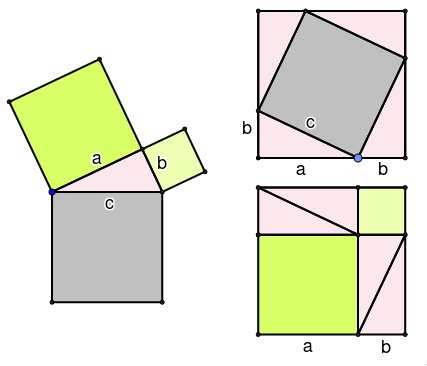
\includegraphics[width=0.5\linewidth]{pictures/dukaz_pythagorovy_vety.png}
    \caption*{Důkaz využívající posunutí}
\end{figure}

\subsubsection*{Euklidova věta o výšce}
Mějme pravoúhlý trojúhelník $ABC$, který má pravý úhel v bodě $C$. Z bodu $C$ vede výška na stranu
$c$, která dělí odvěsnu $c$ na dvě části a to na $c_a$ a $c_b$. Euklidova věta o výšce říká, že 
$v_c^2 = c_a \cdot c_b$.

\begin{figure}[H] 
    \centering    
    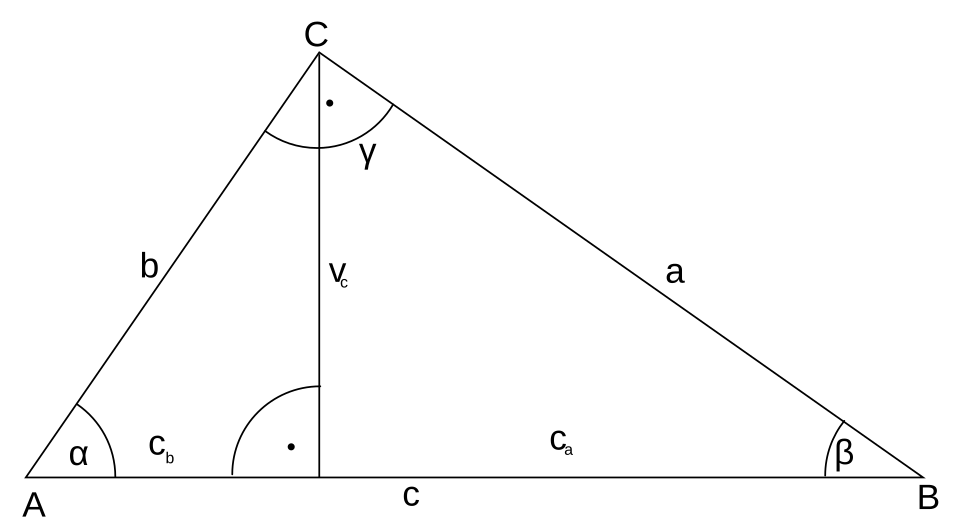
\includegraphics[width=0.5\linewidth]{pictures/euklidova_veta.png}
    \caption*{}
\end{figure}

Pro dokázání Euklidovy věty znovu použijeme podobnost. Označme si patu výšky $v_c$ bodem $P$. Úhel
$\angle CAP$ a $\angle PCB$ mají stejnou velikost a teké úhel $\angle ACP$ a $\angle CBP$ mají také
stejnou velikost. Podle věty uu víme, že tyto trojúhelníky jsou podobné. Podobné trojúhelníky mají
stejný poměr stran, víme tedy, že kratší odvěsna a delší odvěsna budou u obou trojúhelníků ve stejném
poměru. Z toho získáme vzorec $\frac{v_c}{c_a} = \frac{c_b}{v_c}$. Po úpravě získáváme vzorec $v_c^2
= c_a \cdot c_b$
\subsubsection*{Euklidova věta o odvěsně}
Euklidova věta o odvěsně říká, že $a^2 = c \cdot c^a$ a $b^2 = c \cdot c_b$. Pro důkaz využíváme
znovu podobnost. Trojúhelníky $ABC$ a $CPB$ jsou podobné podle věty uu, protože mají úhly se
stejnou velikostí. Poměr přepony a delší odvěsny musí být stejný, tedy platí $\frac{a}{c_a} = \frac{
c}{a}$ a po úpravě získáme $a^2 = c \cdot c_a$. Důkaz pro druhou odvěsnu funguje stejně.

\subsubsection*{Stejnolehlost kružnic}
\begin{center}
\begin{tikzpicture}[line cap=round,line join=round,>=triangle 45,x=1.0cm,y=1.0cm]
\begin{axis}[
x=1.0cm,y=1.0cm,
axis lines=none, 
hide axis,
xmin=-6.2,
xmax=4.5,
ymin=-2.5,
ymax=3.0,
clip=true
]
\definecolor{ududff}{rgb}{0.30,0.30,1}
\draw [line width=0.8pt] (-1.82,-0.78) circle (1.cm);
\draw [line width=0.8pt] (2.14,0.26) circle (2.0cm);
\draw [line width=0.8pt,domain=-10:10] plot(\x,{(--3.7376-1.8413*\x)/-0.7805});
\draw [line width=0.8pt,domain=-10:10] plot(\x,{(-2.7424-1.8413*\x)/-0.7805});
\draw [line width=0.8pt,domain=-10:10] plot(\x,{(-3.4152-1.9606*\x)/-4.3502});
\draw [line width=0.8pt,domain=-10:10] plot(\x,{(--1.196-1.04*\x)/-3.96});
\draw [line width=0.8pt,domain=-10:10] plot(\x,{(-0.3223--3.8020*\x)/5.1308});
\begin{scriptsize}
\fill [ududff] (-1.82,-0.78) circle (2.0pt) node[above right, fill=white, inner sep=0.2pt, xshift=3pt, yshift=2pt] {$S_1$};
\fill [ududff] (2.14,0.26) circle (2.0pt) node[above right, fill=white, inner sep=0.2pt, xshift=3pt, yshift=2pt] {$S_2$};
\fill [ududff] (2.92,2.10) circle (1.8pt) node[above right, fill=white, inner sep=0.2pt, xshift=3pt, yshift=2pt] {$A$};
\fill [ududff] (-1.43,0.14) circle (1.8pt) node[above right, fill=white, inner sep=0.2pt, xshift=3pt, yshift=2pt] {$B$};
\fill [ududff] (-5.78,-1.82) circle (1.8pt) node[above right, fill=white, inner sep=0.2pt, xshift=3pt, yshift=2pt] {$S_{t1}$};
\fill [ududff] (-2.21,-1.70) circle (1.8pt) node[above right, fill=white, inner sep=0.2pt, xshift=3pt, yshift=2pt] {$C$};
\fill [ududff] (-0.5,-0.43) circle (1.8pt) node[above right, fill=white, inner sep=0.2pt, xshift=3pt, yshift=2pt] {$S_{t2}$};
\end{scriptsize}
\end{axis}
\end{tikzpicture}
\end{center}
Dvě kružnice mají dvě stejnolehlosti, vnější a vnitřní. Střed vnější stejnolehlosti je $S_{t1}$ a
střed vnitřní stejnolehlosti je $S_{t2}$. Koeficient stejnolehlosti získáme poměrem poloměrů kružnic a
pro vnější stejnolehlost bude kladný a pro vnitřní záporný. Stejnolehlost kružnic se využívá pro
vytvoření tečny pro obě kružnice zároveň. Vytvoří se středy stejnolehlosti a následně se použije
metoda vytvoření tečny ke kružnici z bodu využitím Thaletovy kružnice.
\subsubsection*{Stejnolehlost úseček}
Dalším častým úkolem je najít středy stejnolehlosti dvou úseček, které leží na jedné přímce.
Tato úloha se dá řešit například vytvořením rovnostranných trojúhelníků. Také to lze řešit
sestrojením dvou kružnic se středy v středech daných úseček a průměrem délky dané úsečky. Středy
stejnolehlosti by se hleadaly stejně jako u hledání tečny ke kružnicím.
\begin{figure}[H]
\centering
\begin{tikzpicture}[scale=0.7, >=stealth]
\draw (-2,0) -- (13,0) node[right] {$p$};
\coordinate (A) at (2.5,0);
\coordinate (B) at (4.5,0);
\draw[ultra thick, blue] (A) -- (B);
\fill[blue] (A) circle (2pt) node[below] {$A$};
\fill[blue] (B) circle (2pt) node[below] {$B$};
\coordinate (C) at (6,0);
\coordinate (D) at (11,0);
\draw[ultra thick, red] (C) -- (D);
\fill[red] (C) circle (2pt) node[below] {$C$};
\fill[red] (D) circle (2pt) node[below] {$D$};
\coordinate (Vab) at (3.5, 1.73); 
\draw[thin, gray] (A) -- (Vab) -- (B);
\fill (Vab) circle (2pt) node[above] {$V_{AB}$};
\coordinate (Vcd) at (8.5, 4.33); 
\draw[thin, gray] (C) -- (Vcd) -- (D);
\fill (Vcd) circle (2pt) node[above] {$V_{CD}$};
\coordinate (Vcd2) at (8.5, -4.33);
\draw[thin, lightgray] (C) -- (Vcd2) -- (D);
\fill[black] (Vcd2) circle (2pt) node[below] {$V'_{CD}$};
\coordinate (S1) at (0.16,0); 
\draw[dashed, blue] (Vcd) -- (S1);
\fill[orange] (S1) circle (3pt) node[below=5pt] {$S_1$};
\coordinate (S2) at (4.93,0); 
\draw[dashed, red] (Vab) -- (Vcd2);
\fill[green!60!black] (S2) circle (3pt) node[below=5pt] {$S_2$};
\end{tikzpicture}
\end{figure}
\end{document}
